\documentclass[10pt,a4paper]{article}

\usepackage[a4paper,margin=2.1cm]{geometry}
\usepackage[T1]{fontenc}
\usepackage{lmodern}
\usepackage{microtype}
\usepackage{amsmath,amssymb}
\usepackage{graphicx}
\usepackage{booktabs}
\usepackage{array}
\usepackage{multirow}
\usepackage{xcolor}
\usepackage{caption}
\usepackage{subcaption}
\usepackage[numbers,sort&compress]{natbib}
\usepackage{tikz}
\usetikzlibrary{positioning,arrows.meta,calc,fit,backgrounds}
\usepackage[colorlinks=true,linkcolor=black,citecolor=black,urlcolor=black]{hyperref}
\usepackage[capitalise,nameinlink]{cleveref}

\captionsetup{font=small,labelfont=bf,skip=4pt}
\setlength{\textfloatsep}{10pt plus 2pt minus 2pt}
\setlength{\floatsep}{8pt plus 2pt minus 2pt}
\setlength{\abovecaptionskip}{3pt}
\setlength{\parskip}{0.25em}

\definecolor{cblue}{HTML}{2a78d6}
\definecolor{corange}{HTML}{eb6834}
\definecolor{caqua}{HTML}{1baf7a}
\definecolor{cgray}{HTML}{52514e}

\newcommand{\pp}{\,pp}
\newcommand{\Pone}{P1}
\newcommand{\Ptwo}{P2}
\newcommand{\Pthree}{P3}

\title{\textbf{Why Neighbour-Consistency Self-Supervision Does Not Help\\Temporal Action Localization:\\A Diagnostic Study with ActionFormer on EPIC-KITCHENS-100}}
\author{[Author name] \\ \small Leiden University \\ \small Master's thesis}
\date{November 2026}

\begin{document}
\maketitle

\begin{abstract}
\noindent
Self-supervised dense objectives such as NeCo, which enforce that the \emph{ordering of
nearest neighbours} of every patch is consistent across augmented views, substantially
improve frozen vision foundation models on dense prediction. We ask whether the same
objective, transplanted from 2D image patches to 1D temporal feature sequences, improves
temporal action localization (TAL). We adapt NeCo to the multi-scale transformer encoder
of ActionFormer, using temporal (and, for VideoMAE, spatial) crops with a 1D ROI-Align,
and evaluate two protocols on the EPIC-KITCHENS-100 verb task with three feature
backbones (SlowFast, VideoMAE-L, V-JEPA~2): self-supervised \emph{post}-training of a
converged supervised model, and self-supervised \emph{pre}-training followed by a full
supervised schedule. Post-training consistently hurts ($-0.52$\pp{} SlowFast, $-0.36$\pp{}
VideoMAE-L average mAP), and jointly re-training the heads does not recover the loss.
Pre-training never produces a gain that exceeds seed noise ($+0.27$\pp{} over three seeds
per arm on SlowFast with a baseline standard deviation of $0.75$\pp; $-0.22$ to $-0.95$\pp{}
across five VideoMAE-L variants; $-0.09$\pp{} on V-JEPA~2). The main contribution is a
diagnosis of \emph{why}. (i) With pre-extracted features, the two temporal views feed
\emph{identical} inputs to 93\% of the finest-level ROI bins, so the invariance NeCo asks
for is largely satisfied by construction. (ii) The objective is absorbed by the projection
head: the encoder moves $\sim$50$\times$ less than under supervised training, and because
the EMA teacher's time constant (2000 steps) exceeds the whole run (1476 steps), the
encoder that is actually transferred moves only 0.08\% from its random initialisation,
$\sim$300$\times$ less than supervised training does. Pre-training is thus, to first order,
a $10^{-3}$ perturbation of the baseline's initialisation. (iii) Supervised training
erases whatever remains: the resulting encoders are as similar to the baseline as two
baseline seeds are to each other, and the SSL initialisation gives no head start in the
supervised loss. (iv) When the encoder \emph{is} made to move (stronger SSL schedule,
or post-training), the downstream result gets worse. A control experiment in NeCo's own
setting (DINOv2 $\rightarrow$ PASCAL VOC) reproduces its published gain ($+2.0$ mIoU),
showing that the null result is a property of applying the objective to frozen,
already-supervised clip features for a sparse temporal task, not of the objective itself.
\end{abstract}

%=======================================================================================
\section{Introduction}
%=======================================================================================

Temporal action localization (TAL) asks a model to find \emph{when} each action in an
untrimmed video starts and ends and \emph{what} it is. Modern single-stage detectors such
as ActionFormer~\cite{zhang2022actionformer} operate on pre-extracted clip features: a
frozen video backbone (e.g.\ SlowFast~\cite{feichtenhofer2019slowfast} or
VideoMAE~\cite{tong2022videomae}) turns a video into a sequence of feature vectors, and a
light multi-scale transformer encoder followed by classification and regression heads is
trained on top. The encoder is the only part of this pipeline that learns temporal
context, and it is trained from scratch on a few hundred labelled videos.

Self-supervised learning (SSL) is the standard answer to scarce labels. Among dense SSL
objectives, NeCo~\cite{pariza2025neco} is attractive for localization: rather than making
whole-image embeddings invariant, it asks that every patch rank a set of reference patches
in the same order in two augmented views. Applied as a short post-training stage on
DINOv2~\cite{oquab2024dinov2}, it gives consistent gains on semantic segmentation. Because
the ActionFormer encoder is, structurally, a dense per-timestep feature extractor over a
1D sequence, the analogy is direct: temporal positions play the role of patches and
temporal crops the role of image crops. If neighbourhood consistency helps patches find
the right semantic neighbours, it might help timesteps find the right action neighbours.

This thesis tests that analogy and reports a negative result: \textbf{NeCo-style SSL does
not improve ActionFormer on EPIC-KITCHENS-100 verbs}, neither as post-training nor as
pre-training, on any of three feature backbones. Negative results are only useful if
their cause is understood, so most of the work goes into the diagnosis. Our contributions are:
\begin{itemize}\setlength\itemsep{0pt}
\item A 1D adaptation of NeCo to ActionFormer's encoder (temporal crops, multi-scale
  1D ROI-Align, cross-video reference pools, an EMA teacher), with temporal, spatial,
  spatio-temporal and frame-rate view variants, and an \texttt{--init-encoder} path that
  transfers the SSL encoder into the unmodified supervised recipe (\cref{sec:method}).
\item A controlled evaluation of post-training and pre-training on SlowFast, VideoMAE-L and
  V-JEPA~2 features, with seed replicates and a joint fine-tuning ablation with a matched
  control (\cref{sec:results}).
\item A mechanistic explanation of the null result from four independent angles: view
  identity in input space, weight movement of the transferred encoder (including an EMA
  lag that makes the transferred encoder almost exactly the random initialisation),
  representation similarity after fine-tuning, and the effect of forcing the encoder to
  train more (\cref{sec:why}).
\item A positive control showing that NeCo does work in its own setting under the same
  measurement protocol, which localizes the failure to the TAL setting rather than to
  the objective (\cref{sec:voc}).
\end{itemize}

%=======================================================================================
\section{Related Work}
%=======================================================================================

\paragraph{Temporal action localization.}
Early proposal-based methods such as BMN~\cite{lin2019bmn} and
G-TAD~\cite{xu2020gtad} were overtaken by single-stage transformer detectors.
ActionFormer~\cite{zhang2022actionformer} combines a convolutional embedding, a
multi-scale transformer with local self-attention, and per-timestep classification and
boundary regression heads; TriDet~\cite{shi2023tridet} and many later methods keep this
backbone and change the heads. Nearly all of these operate on frozen features, and much
of the recent progress has come from better features, e.g.\ EPIC-finetuned VideoMAE, or from
end-to-end backbone adaptation~\cite{liu2024adatad,liu2025opentad}.

\paragraph{Self-supervised dense representation learning.}
Joint-embedding SSL learns invariances to the augmentations used to create
views~\cite{chen2020simclr,grill2020byol,caron2021dino}; which invariances are learned is
determined almost entirely by how the views differ~\cite{tian2020goodviews}. Dense
variants transfer this idea from images to patches. Leopart~\cite{ziegler2022leopart}
clusters patch features, and NeCo~\cite{pariza2025neco} replaces patch-to-prototype
matching with a differentiable sort~\cite{prillo2020softsort} of patch-to-reference
distances, aligning the two views with ROI-Align~\cite{he2017maskrcnn} and using an EMA
teacher~\cite{tarvainen2017meanteacher}.

\paragraph{Pre-training for localization.}
Localization-specific pre-training of the \emph{video backbone}, such as
TSP~\cite{alwassel2021tsp} and BSP~\cite{xu2021bsp}, improves TAL by changing the features
themselves. Our setting is different: the backbone and its features are fixed, and only
the TAL encoder on top is pre-trained. Results from image recognition suggest caution
here. He et al.~\cite{he2019rethinking} found that with a full training schedule,
ImageNet pre-training mainly speeds up convergence and does not improve final accuracy,
and Raghu et al.~\cite{raghu2019transfusion} found that much of what transfer learning
provides is weight scaling rather than reusable features. We measure the analogous
quantities directly, using weight movement and linear CKA~\cite{kornblith2019cka}.

%=======================================================================================
\section{Method}\label{sec:method}
%=======================================================================================

\subsection{ActionFormer}
A video is represented by a sequence of frozen clip features $X\in\mathbb{R}^{T\times C}$
(SlowFast: $C{=}2304$, one vector every 16 frames at 30\,fps, i.e.\ 1.875 vectors/s).
The encoder $f_\theta$ consists of two 1D convolutions (kernel 3), two transformer blocks,
and five further transformer blocks that each halve the temporal resolution, producing a
six-level feature pyramid $\{F^{(l)}\}_{l=0}^{5}$ with stride $2^l$ and 512 channels. All
self-attention is local with a window of 9 positions. An identity neck passes the pyramid to
shared classification and regression heads, trained with focal~\cite{lin2017focal} and
DIoU~\cite{zheng2020diou} losses and center sampling. At inference, Soft-NMS~\cite{bodla2017softnms}
merges candidates from all levels. The encoder (``backbone + neck'', 207 parameter tensors)
is the only component shared by every pipeline below; only the heads (22 tensors)
differ.

\subsection{NeCo on a temporal feature sequence}\label{sec:neco1d}

\begin{figure}[t]
\centering
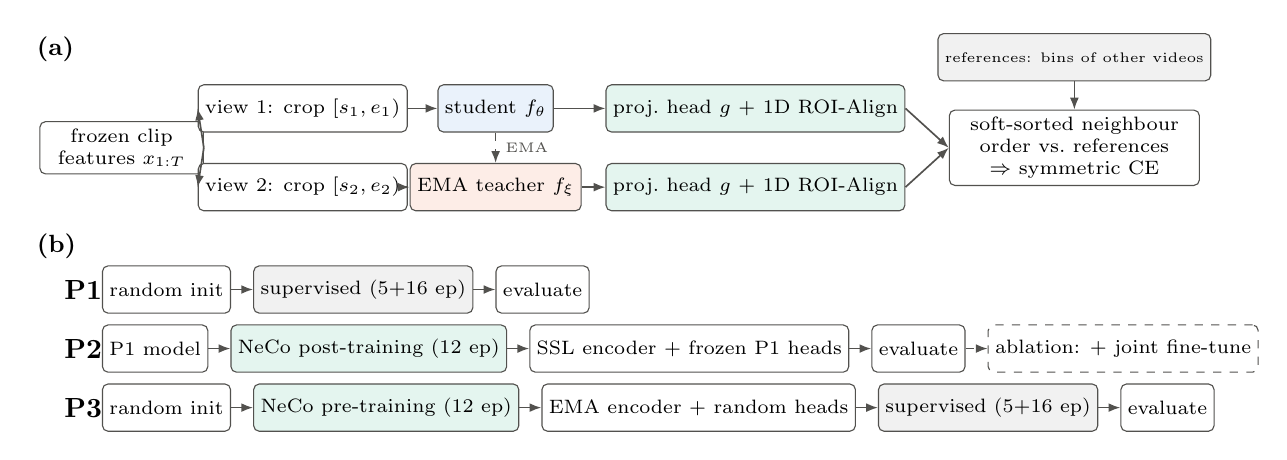
\begin{tikzpicture}[font=\scriptsize,
  box/.style={draw=cgray, rounded corners=2pt, align=center, inner sep=2.5pt, minimum height=0.6cm, fill=white},
  sbox/.style={box, fill=cblue!10}, tbox/.style={box, fill=corange!12}, hbox/.style={box, fill=caqua!12},
  arr/.style={-{Latex[length=1.5mm]}, semithick, cgray}]
% ---------------- (a) objective
\node[font=\small\bfseries, anchor=west] at (-0.2, 0.75) {(a)};
\node[box, text width=1.9cm] (x) at (1.0,-0.5) {frozen clip features $x_{1:T}$};
\node[box] (v1) at (3.3, 0.0) {view 1: crop $[s_1,e_1)$};
\node[box] (v2) at (3.3,-1.0) {view 2: crop $[s_2,e_2)$};
\node[sbox] (s) at (5.75, 0.0) {student $f_\theta$};
\node[tbox] (t) at (5.75,-1.0) {EMA teacher $f_\xi$};
\node[hbox] (g1) at (9.05, 0.0) {proj.\ head $g$ + 1D ROI-Align};
\node[hbox] (g2) at (9.05,-1.0) {proj.\ head $g$ + 1D ROI-Align};
\node[box, text width=3.0cm] (L) at (13.1,-0.5) {soft-sorted neighbour\\order vs.\ references\\$\Rightarrow$ symmetric CE};
\node[box, font=\tiny, fill=cgray!8] (R) at (13.1, 0.65) {references: bins of other videos};
\draw[arr] (x.east) -- (v1.west); \draw[arr] (x.east) -- (v2.west);
\draw[arr] (v1) -- (s); \draw[arr] (v2) -- (t);
\draw[arr] (s) -- (g1); \draw[arr] (t) -- (g2);
\draw[arr] (g1.east) -- (L.west); \draw[arr] (g2.east) -- (L.west); \draw[arr] (R) -- (L);
\draw[arr, dashed] (s) -- node[right, font=\tiny]{EMA} (t);
% ---------------- (b) protocols
\node[font=\small\bfseries, anchor=west] at (-0.2,-1.75) {(b)};
\def\gap{0.28cm}
\node[font=\bfseries, anchor=west] at (0.15,-2.3) {P1};
\node[box, anchor=west] (p1a) at (0.75,-2.3) {random init};
\node[box, right=\gap of p1a, fill=cgray!8] (p1b) {supervised (5+16 ep)};
\node[box, right=\gap of p1b] (p1c) {evaluate};
\draw[arr] (p1a) -- (p1b); \draw[arr] (p1b) -- (p1c);
\node[font=\bfseries, anchor=west] at (0.15,-3.05) {P2};
\node[box, anchor=west] (p2a) at (0.75,-3.05) {P1 model};
\node[box, right=\gap of p2a, fill=caqua!12] (p2b) {NeCo post-training (12 ep)};
\node[box, right=\gap of p2b] (p2c) {SSL encoder + frozen P1 heads};
\node[box, right=\gap of p2c] (p2d) {evaluate};
\node[box, right=\gap of p2d, dashed] (p2e) {ablation: + joint fine-tune};
\draw[arr] (p2a) -- (p2b); \draw[arr] (p2b) -- (p2c); \draw[arr] (p2c) -- (p2d); \draw[arr, dashed] (p2d) -- (p2e);
\node[font=\bfseries, anchor=west] at (0.15,-3.8) {P3};
\node[box, anchor=west] (p3a) at (0.75,-3.8) {random init};
\node[box, right=\gap of p3a, fill=caqua!12] (p3b) {NeCo pre-training (12 ep)};
\node[box, right=\gap of p3b] (p3c) {EMA encoder + random heads};
\node[box, right=\gap of p3c, fill=cgray!8] (p3d) {supervised (5+16 ep)};
\node[box, right=\gap of p3d] (p3e) {evaluate};
\draw[arr] (p3a) -- (p3b); \draw[arr] (p3b) -- (p3c); \draw[arr] (p3c) -- (p3d); \draw[arr] (p3d) -- (p3e);
\end{tikzpicture}
\caption{\textbf{(a)} NeCo adapted to 1D. Two overlapping crops of the same pre-extracted
feature sequence are encoded by a student and an EMA teacher. Every pyramid level is
projected and ROI-aligned onto the crop intersection, and the loss asks the ordering of
reference bins (drawn from the other videos in the batch) to agree between the two
views. \textbf{(b)} The three protocols. P1 is the supervised baseline. P2 post-trains
the encoder of a converged P1 model and splices it back onto the frozen P1 heads. P3
runs SSL from a random initialisation and transfers the EMA encoder into the
unmodified supervised recipe; only the encoder's starting point differs from P1.}
\label{fig:method}
\end{figure}

\paragraph{Views.} Following NeCo, each training sample yields two views, but here they
are crops of a 1D sequence (\cref{fig:method}a). For a video of $T$ feature steps
(randomly windowed to the encoder's maximum length if longer), two crop lengths are drawn
uniformly from $[\max(0.4T, 128), T]$ and the crops are placed so that they overlap by at
least 20\% of the shorter one. Their intersection $[\max(s_1,s_2), \min(e_1,e_2))$ is the
shared region of interest (ROI). The student encodes view~1 and the teacher view~2.

\paragraph{Projection and alignment.} At every pyramid level, a 3-layer position-wise MLP
$g$ (512$\to$2048$\to$2048$\to$256, GELU, dropout 0.1) projects the features. A 1D
ROI-Align then linearly interpolates them at $N{=}32$ equally spaced bin centres in
the ROI, expressed in each view's own coordinates and the level's stride. The six aligned
levels are concatenated, fused by a linear mixer with LayerNorm, and L2-normalised, giving
anchors $z^{s}_{b,n}$ (student) and $z^{t}_{b,n}$ (teacher) for video $b$ and bin $n$.

\paragraph{Neighbour-order loss.} For video $b$, the reference set $O_b=\{o_r\}_{r=1}^{R}$
contains a random half of the valid student bins of every \emph{other} video in the batch
(stop-gradient; $R=48$ for batch size 4). With distances $d^{v}_{n,r}=-\langle z^{v}_{b,n},
o_r\rangle$ for $v\in\{s,t\}$, SoftSort~\cite{prillo2020softsort} gives a differentiable
rank $\rho^{v}_{n,r}=\sum_{j}\sigma\big((d^{v}_{n,r}-d^{v}_{n,j})/\tau_r\big)$ and a soft
permutation matrix
\begin{equation}
P^{v}_{n}[k,r]=\operatorname{softmax}_r\!\Big(-\frac{|k-\rho^{v}_{n,r}|}{\tau_p}\Big),
\qquad k=0,\dots,R-1,
\end{equation}
i.e.\ the probability that reference $r$ is the $k$-th nearest neighbour of anchor $n$.
The loss is the symmetric cross-entropy between the two views' soft permutations,
\begin{equation}
\mathcal{L}_{\text{NeCo}}=\frac{1}{|\mathcal{A}|}\sum_{(b,n)\in\mathcal{A}}\frac{1}{R}
\Big[\operatorname{CE}\big(P^{t}_{n},P^{s}_{n}\big)+\operatorname{CE}\big(P^{s}_{n},P^{t}_{n}\big)\Big],
\quad \operatorname{CE}(P,Q)=-\sum_{k,r}P[k,r]\log Q[k,r],
\end{equation}
with $\tau_r=\tau_p=0.1$. We also log the \emph{top-1 agreement}: the fraction of anchors
whose nearest reference is the same in both views. The teacher is an exponential moving
average $\xi\leftarrow m\,\xi+(1-m)\,\theta$ whose momentum follows a cosine schedule from
$m_0=0.9995$ to 1 over the run.

\paragraph{View variants.} Besides temporal crops, we test: \emph{frame-rate
augmentation}, where each view is resampled at a rate $r\sim\text{log-}\mathcal{U}[0.5,2]$
and the ROI is mapped with stride $\times r$; \emph{spatial crops} for VideoMAE-L, where
16 spatial crops per snippet are re-extracted from the backbone's dense tokens and pooled,
so that the two views cover the same time span but see different image regions; and the
combination of spatial crops with random temporal crops.

\subsection{Protocols}
\Cref{fig:method}b summarises the three protocols. \textbf{P1} is the supervised
baseline. \textbf{P2 (post-training)} warm-starts the encoder from the converged P1
model, trains it with $\mathcal{L}_{\text{NeCo}}$, and evaluates the EMA encoder spliced
onto the frozen P1 heads. A follow-up ablation then fine-tunes encoder and heads jointly
with the supervised loss (1 warm-up + 5 cosine epochs, lr $2{\times}10^{-5}$), and a control
applies the identical fine-tune to the unmodified P1 model. \textbf{P3 (pre-training)},
the order used in the SSL literature, runs $\mathcal{L}_{\text{NeCo}}$ from a random
initialisation (stage~A), loads only the backbone and neck from the SSL checkpoint's EMA
teacher, and trains the whole model with the unmodified P1 recipe (stage~B). In P3 the
encoder initialisation is the only difference from P1.

%=======================================================================================
\section{Experimental Setup}\label{sec:setup}
%=======================================================================================

\paragraph{Data and features.} EPIC-KITCHENS-100~\cite{damen2022epic}, verb task
(97 classes): 495 training and 138 validation videos of egocentric kitchen activity,
evaluated on the validation split. We use three frozen feature tracks: (i)
\textbf{SlowFast}, the official EPIC-pretrained features used by
ActionFormer (2304-d, 32-frame windows, stride 16); (ii) \textbf{VideoMAE-L} fine-tuned on
EPIC verbs, as released by OpenTAD~\cite{liu2025opentad} (1024-d, 16-frame windows, stride
8, twice the SlowFast density); and (iii) \textbf{V-JEPA~2} ViT-L~\cite{assran2025vjepa2},
frozen and not adapted to EPIC (1024-d, density matched to SlowFast).

\paragraph{Training.} \Cref{tab:hparams} lists the schedules. Supervised training is the
published ActionFormer recipe and is identical in P1 and P3 stage~B. The SSL ``v1''
schedule was used for all runs except one VideoMAE-L run (``v2''), which raises the encoder
learning rate, removes the 10$\times$ head learning-rate multiplier, relaxes gradient
clipping and trains longer, to test whether the encoder was simply under-trained.

\begin{table}[t]
\centering\small
\caption{Training schedules. One SSL epoch is 123 iterations (batch 4).}
\label{tab:hparams}
\begin{tabular}{lccc}
\toprule
 & Supervised (P1, P3-B) & SSL v1 (P2, P3-A) & SSL v2 (VideoMAE-L) \\
\midrule
epochs (warm-up + main) & 5 + 16 & 2 + 10 & 2 + 18 \\
optimizer, batch size & AdamW, 2 & AdamW, 4 & AdamW, 4 \\
encoder learning rate & $1{\times}10^{-4}$ & $2{\times}10^{-5}$ & $1{\times}10^{-4}$ \\
head learning rate & $1{\times}10^{-4}$ & $2{\times}10^{-4}$ (10$\times$) & $1{\times}10^{-4}$ (1$\times$) \\
grad.\ clip (global L2) & 1.0 & 1.0 & 5.0 \\
EMA momentum & 0.999 (eval.\ model) & $0.9995\rightarrow1$ (teacher) & $0.9995\rightarrow1$ (teacher) \\
\bottomrule
\end{tabular}
\end{table}

\paragraph{Evaluation and statistics.} We report mAP at temporal IoU
$\{0.1,\dots,0.5\}$ and their average (``avg mAP''), from the EMA model after the final
epoch. Seed replicates exist for the SlowFast baseline and SlowFast P3 (seeds 0, 1, 2;
for P3 both stages are re-seeded). Every other row is a single run. We therefore use the
SlowFast baseline's seed standard deviation, 0.75\pp, as the noise scale for single-run
differences on all tracks.

\paragraph{Diagnostics.} \emph{Weight movement} is
$\|W-W_0\|_2/\|W_0\|_2$ per parameter group, where $W_0$ is re-created from the run's seed.
\emph{Linear CKA}~\cite{kornblith2019cka} compares the pyramid features two encoders
produce on the same 40--60 validation videos, averaged over levels. It is invariant to
rotations of feature space, so we interpret it against a control: two independently seeded
baselines.

%=======================================================================================
\section{Results}\label{sec:results}
%=======================================================================================

\begin{table}[t]
\centering\small
\caption{EPIC-KITCHENS-100 verb, validation mAP (\%). Mean $\pm$ sample sd where $n{=}3$.
Rows without $\pm$ are single runs. P2 rows are compared with the model they start from
(23.07) or with the matched control (22.97).}
\label{tab:main}
\setlength{\tabcolsep}{5pt}
\begin{tabular}{llcccccc}
\toprule
Features & Model & 0.1 & 0.2 & 0.3 & 0.4 & 0.5 & Avg \\
\midrule
\multirow{8}{*}{SlowFast}
 & ActionFormer (paper~\cite{zhang2022actionformer}) & 26.6 & 25.4 & 24.2 & 22.3 & 19.1 & 23.5 \\
 & P1 baseline ($n{=}3$) & 26.67 & 25.51 & 24.16 & 21.98 & 18.58 & 23.38\,$\pm$\,0.75 \\
 & \quad P1, seed 0 (source of P2) & 26.40 & 25.15 & 23.73 & 21.70 & 18.35 & 23.07 \\
 & P2 post-training, frozen heads & 26.14 & 24.70 & 23.20 & 20.93 & 17.79 & 22.55 \\
 & P2 + joint fine-tune & 26.15 & 24.78 & 23.14 & 21.21 & 17.83 & 22.45 \\
 & \quad control: P1 + same fine-tune & 26.41 & 25.16 & 23.55 & 21.52 & 18.22 & 22.97 \\
 & P3 pre-training ($n{=}3$) & 26.81 & 25.81 & 24.45 & 22.34 & 18.86 & 23.65\,$\pm$\,0.08 \\
 & P3 + frame-rate augmentation & 27.92 & 26.68 & 25.15 & 22.79 & 19.70 & 24.45 \\
\midrule
\multirow{6}{*}{VideoMAE-L}
 & P1 baseline & 32.84 & 32.06 & 30.42 & 28.11 & 24.59 & \textbf{29.60} \\
 & P2 post-training, frozen heads & 32.65 & 31.80 & 29.96 & 27.83 & 23.97 & 29.24 \\
 & P3, temporal crops & 32.83 & 32.23 & 30.58 & 27.84 & 23.46 & 29.38 \\
 & P3, spatial crops & 32.65 & 32.01 & 30.41 & 27.78 & 24.05 & 29.38 \\
 & P3, spatial + temporal crops & 32.44 & 31.61 & 29.58 & 27.23 & 23.65 & 28.90 \\
 & P3, spatial crops, SSL v2 & 31.62 & 30.97 & 29.35 & 27.28 & 24.03 & 28.65 \\
\midrule
\multirow{2}{*}{V-JEPA 2}
 & P1 baseline & 20.51 & 19.74 & 18.38 & 16.17 & 12.64 & 17.49 \\
 & P3, temporal crops & 20.33 & 19.49 & 18.11 & 15.87 & 13.19 & 17.40 \\
\bottomrule
\end{tabular}
\end{table}

\begin{figure}[t]
\centering
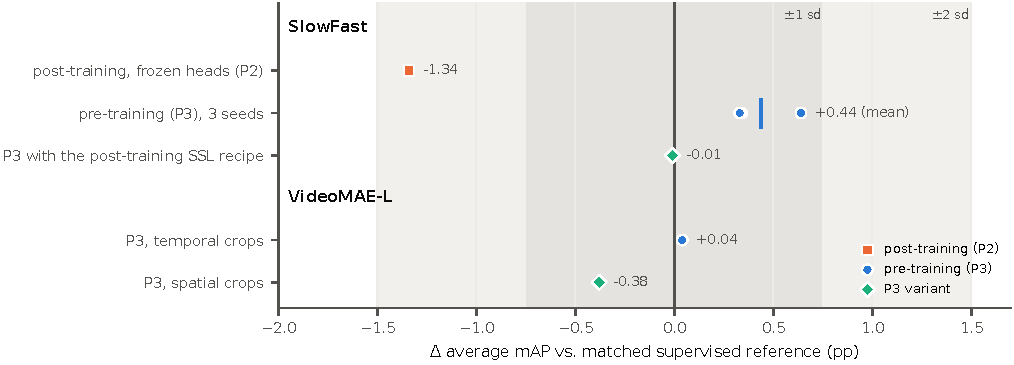
\includegraphics[width=\linewidth]{figs/fig_results.pdf}
\caption{Every SSL variant as a difference in average mAP to its matched supervised
reference. Shaded bands: $\pm1$ and $\pm2$ standard deviations of the SlowFast baseline
over seeds (0.75\pp). This is the only measured noise scale and is applied to all tracks.
Post-training (squares) is below its reference on both tracks it was run on. No
pre-training variant leaves the $\pm2$\,sd band.}
\label{fig:results}
\end{figure}

\Cref{tab:main} gives all results and \cref{fig:results} shows each variant against its
reference. Our SlowFast reproduction (23.38\,$\pm$\,0.75 over three seeds; range
22.84--24.23) brackets the published 23.5, so the pipeline is sound. Feature choice
dominates everything else: VideoMAE-L is 6.2\pp{} above SlowFast and 12.1\pp{} above
frozen V-JEPA~2. Every SSL effect below is at least an order of magnitude smaller.

\paragraph{Post-training hurts, and the damage is in the encoder.} P2 lowers SlowFast
from 23.07 to 22.55 ($-0.52$\pp) and VideoMAE-L from 29.60 to 29.24 ($-0.36$\pp), at every
tIoU threshold on SlowFast, with the largest drop at the stricter thresholds. The SSL
objective itself converges (top-1 agreement $0.57\rightarrow0.83$), so this is a transfer
failure, not an optimization failure. An obvious suspect is \emph{head mismatch}: the
frozen heads no longer fit the drifted encoder. The joint fine-tune rules this out.
After six epochs of joint training the post-trained model is still at 22.45--22.61, while
the control given the same epochs stays at 22.94--23.02. The gap stays at $\sim$0.5\pp{} in
every epoch (\cref{fig:trajectories}c), so within this budget the post-trained encoder
cannot be steered back. The damage is in the encoder, not in the encoder--head
interface.

\paragraph{Pre-training does not raise mAP.} On a single seed, SlowFast P3 looked like a
gain (23.56 vs.\ 23.07). With three seeds per arm the difference of means is $+0.27$\pp{}
(Welch $t\approx0.6$, $p\approx0.6$), well inside the baseline's own spread. There is no
gain on V-JEPA~2 ($-0.09$) and none on VideoMAE-L, where all five SSL variants land between
$-0.22$ and $-0.95$\pp. The variants differ in view type (temporal, spatial, combined) and
in how hard the encoder is trained (v2). The VideoMAE-L baseline is a single run, so a
consistently negative sign may partly reflect a baseline that happened to draw high.
Either way, there is no evidence of a gain.

\paragraph{Two apparent positives.} Two observations could be read as SSL benefits. The
three P3 seeds are much tighter than the baseline seeds (sd 0.08 vs.\ 0.75; nominal
two-sided F-test $p\approx0.02$ with 2 and 2 degrees of freedom). The frame-rate-augmented
run reaches 24.45, the best SlowFast number in the study. \Cref{sec:why-perturb} shows that
neither can be attributed to SSL: all of these runs start from essentially the same
weights.

\begin{figure}[t]
\centering
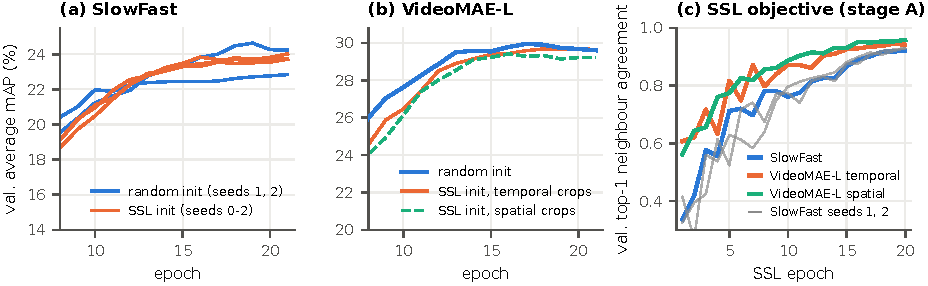
\includegraphics[width=\linewidth]{figs/fig_trajectories.pdf}
\caption{Validation average mAP during training. \textbf{(a)} SlowFast: the baseline seeds
(blue) and P3 seeds (orange) overlap throughout, and the run-to-run spread is as large as
any gap between protocols. \textbf{(b)} VideoMAE-L: SSL-initialised runs track the
baseline and end slightly below it. \textbf{(c)} Joint fine-tune after post-training
(epoch 0 = before fine-tuning): the $\sim$0.5\pp{} gap to the control does not close.}
\label{fig:trajectories}
\end{figure}

\Cref{fig:trajectories} shows that SSL initialisation does not change the shape of
training either. The curves of the two arms overlap from the first epoch on.

%=======================================================================================
\section{Why NeCo Pre-Training Does Not Help}\label{sec:why}
%=======================================================================================

The results leave two questions: why pre-training changes nothing, and why
post-training makes things worse. We approach them in the order in which information
flows through the pipeline: what the views contain, what the SSL stage changes, what
survives supervised training, and what happens when the encoder is forced to change.

\subsection{An upper bound: SSL cannot add information}\label{sec:why-info}
The clip features are computed once by a frozen backbone and are byte-identical in every
run; no code path rewrites them. SSL and supervised training therefore see exactly the
same tensors from exactly the same 495 videos, and by the data-processing
inequality~\cite{cover2006elements} no function of those tensors can contain more
information about the actions than the tensors themselves. The SSL stage can only
change \emph{where the encoder starts} when it learns to combine a fixed representation.
For features already fine-tuned on EPIC verbs (VideoMAE-L) or pre-trained on EPIC
(SlowFast), that representation is already strongly verb-discriminative. This bounds the
achievable gain but does not by itself predict zero: a better starting point could still
help optimisation or generalisation. The next sections show why it does not here.

\subsection{The two temporal views are mostly the same input}\label{sec:why-views}

\begin{figure}[t]
\centering
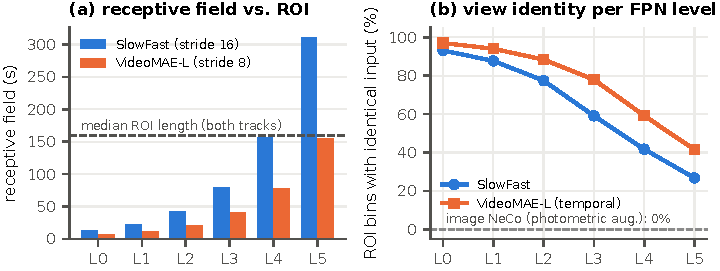
\includegraphics[width=0.78\linewidth]{figs/fig_views.pdf}
\caption{View identity under temporal cropping, computed by running the training crop
sampler on the true EPIC training-video lengths (40 crop pairs per video).
\textbf{(a)} Receptive field of each pyramid level in seconds, against the median ROI
length. \textbf{(b)} Fraction of ROI bins whose entire receptive field lies within
both crops, i.e.\ where the two views give the encoder byte-identical input. In
image NeCo, colour jitter, blur and rescaling change every pixel, so this fraction is 0.}
\label{fig:views}
\end{figure}

In image NeCo the two views of a patch differ in scale, colour, blur and context. Joint-embedding
methods learn exactly the invariances encoded by these differences~\cite{chen2020simclr,tian2020goodviews}.
With pre-extracted clip features, pixel-level augmentations are impossible, and temporal
cropping changes only the \emph{context} around a position, not the position's input. A
ROI bin at position $p$ on level $l$ receives identical input in both views whenever its
receptive field $[p-r_l,p+r_l]$ is cut identically by both crops. From the architecture, $r_l$
is 12, 21, 39, 75, 147 and 291 feature steps for levels 0--5. Running the actual crop
sampler on the true video lengths (\cref{fig:views}) shows that, for SlowFast,
\textbf{93\% of level-0 bins and 77\% of level-2 bins see identical inputs in both views}.
Only the coarsest levels, whose receptive fields (up to 5\,min) exceed the median ROI
($\sim$160\,s), see substantially different context. VideoMAE-L is even more extreme (97\%
at level 0) because its finer stride gives each level a shorter receptive field in seconds.
(This is an upper bound on identical \emph{outputs}: at levels $\ge 1$ the two views'
sampling grids can be offset by a fraction of the stride, and stochastic depth adds noise.)

The consequence is that for most anchors the student and teacher already receive the
same input, so neighbour-order consistency is satisfied by \emph{any} encoder, random or
trained, up to the teacher--student weight difference. The learning signal comes only from
the minority of bins near the ROI boundary and from the coarse levels, and what it teaches
is invariance to \emph{distant} context. Nothing in this signal tells the encoder which
moments belong to the same action. The frame-rate and spatial-crop variants were designed
to make the inputs differ, but they did not change the downstream outcome either
(\cref{tab:main}), which points to the optimisation analysis below as the binding
constraint.

\subsection{The objective is absorbed by the head, and the transferred encoder barely moves}\label{sec:why-move}

\begin{figure}[t]
\centering
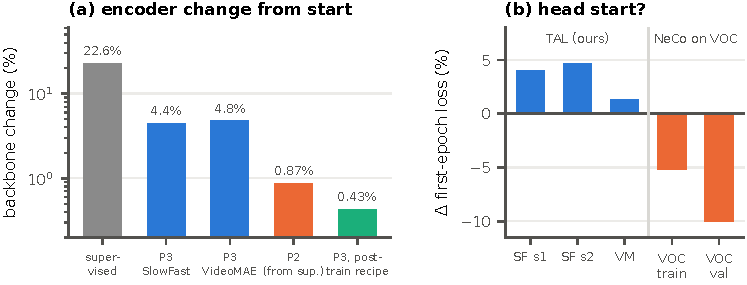
\includegraphics[width=\linewidth]{figs/fig_movement.pdf}
\caption{\textbf{(a)} Relative weight change from the random initialisation (log scale).
Supervised training moves the backbone by 24\%. SSL v1 moves the student backbone by
0.47\% and the projection head by 12\%, and the EMA teacher, which is what P3 transfers,
moves by only 0.08\%. \textbf{(b)} Simulated EMA tracking of a student whose displacement
follows the learning-rate schedule (dotted), under the cosine momentum schedule from
$m_0{=}0.9995$. Stars: measured teacher/student ratios, which match the simulation.
\textbf{(c)} The SSL objective is fit well in every run (top-1 neighbour agreement on
validation).}
\label{fig:movement}
\end{figure}

\paragraph{The projection head does the work.} \Cref{fig:movement}a measures how far each
part of the model moves during SSL. The objective is fit well (\cref{fig:movement}c:
agreement 0.77--0.89, NeCo loss $\sim$14$\rightarrow$2.2), but almost all of the change
happens in the projection head: 12\% relative change, against 0.47\% for the student
backbone and 0.05\% for the neck. Supervised training moves the same backbone by 24\%,
about 50$\times$ more. Three properties of the v1 schedule favour this outcome, and all
three are inherited from the image recipe. The head's learning rate is 10$\times$ the
encoder's. Gradient clipping is global, so the head's large gradients use up the clipping
budget. And a 3-layer, 2048-wide MLP applied to identical inputs (\cref{sec:why-views})
can satisfy the ranking target without any help from below. The mixer that fuses
pyramid levels does not learn a shortcut either: its per-level weight norms change by at
most 3\% and stay nearly uniform across levels.

\paragraph{The EMA teacher lags so much that it barely leaves the initialisation.} P3
transfers the EMA \emph{teacher}, the usual choice because the teacher is the converged,
less noisy copy. Its momentum starts at $m_0=0.9995$, a time constant of
$1/(1-m_0)=2000$ steps, and rises towards 1. The whole v1 run is only 1476 steps (12 epochs
of 123 iterations), so the teacher cannot catch up with the student. A simulation of the
schedule predicts that the teacher captures 13\% of the student's final displacement in
v1 and 23\% in v2 (\cref{fig:movement}b). The measured ratios are 17\% and 30\%. The
transferred backbone has therefore moved only \textbf{0.08\%} from its random
initialisation, about 300$\times$ less than supervised training moves it. The same
holds for every v1 run (SlowFast, VideoMAE-L temporal and spatial, frame-rate augmentation,
and the other seeds all measure 0.079--0.082\%). This schedule was designed for image
SSL runs that are tens of thousands of steps long. On a dataset of 495 videos it all but
freezes the teacher.

\paragraph{Consequence: P3 is the baseline with a $10^{-3}$ perturbation.}\label{sec:why-perturb}
Both arms use the same initialisation seed, and stage~B builds its heads exactly as P1
does. So for a given seed, P3 starts from the P1 initialisation with a relative encoder
perturbation of $\sim$$8\times10^{-4}$. This is visible in the supervised loss: the first
minibatch loss of seed-matched pairs agrees to within 0.4\% (e.g.\ 1.9725 vs.\ 1.9762).
This reframes the comparisons in \cref{sec:results}. The paired differences between P3
and P1 for the same seed ($+0.49$, $+0.83$, $-0.51$\pp) do not measure SSL. They measure
how much a $10^{-3}$ perturbation of the starting point changes the end of a 21-epoch
run with batch size 2, and the answer, up to 0.8\pp, is about the same as the
seed-to-seed spread. The frame-rate-augmented run (24.45) shares its seed with P3 seed~0
(23.56) and P1 seed~0 (23.07). All three runs start within $10^{-3}$ of the same weights,
so their 1.4\pp{} range is a direct estimate of this perturbation noise, and the 24.45
cannot be credited to the augmentation. The same reasoning applies to the low P3 spread
across seeds: three near-random initialisations have no mechanism for being more stable
than three random ones. With $n{=}3$ and many comparisons made in this study, we read it
as chance.

\subsection{Supervised training erases the initialisation}\label{sec:why-erase}

\begin{figure}[t]
\centering
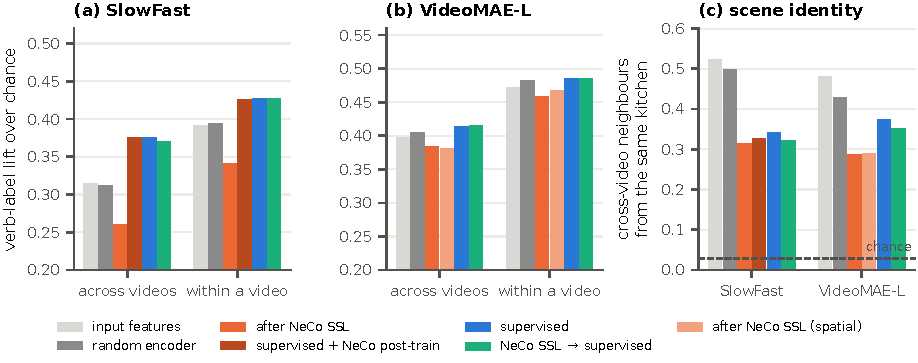
\includegraphics[width=\linewidth]{figs/fig_representation.pdf}
\caption{\textbf{(a)} Linear CKA between encoder representations on validation videos.
The SSL stage-A encoder is no closer to a trained supervised encoder than a random
initialisation is. After supervised training, the SSL-initialised encoder is exactly
as similar to a baseline of a different seed (0.90) as two baseline seeds are to each other
(0.90, dashed). The higher same-seed values reflect the shared initialisation.
\textbf{(b)} Epoch-1 supervised loss of the SSL-initialised run minus the random-initialised
run (mean over minibatches $\pm$ paired s.e.). There is no head start. \textbf{(c)} VideoMAE-L:
a better fit of the SSL objective does not give a better detector. v2, whose encoder moves
20$\times$ more, is the worst.}
\label{fig:representation}
\end{figure}

Even setting the EMA lag aside, the student encoder moves only 0.5\%, and supervised
training then moves it by another 24\%. \Cref{fig:representation}a shows that nothing
distinctive survives. Before supervised training, the SSL encoder is no closer to the
supervised representation than a random initialisation (CKA 0.49 vs.\ 0.49 on SlowFast,
0.66 vs.\ 0.62 on VideoMAE-L). After supervised training, the SSL-initialised encoder and a
baseline with a \emph{different} seed have CKA 0.896, the same as two baseline seeds (0.899).
The supervised objective, not the initialisation, determines the final representation, in
line with the observation of He et al.~\cite{he2019rethinking} that full schedules wash out
pre-training. Here not even the convergence-speed benefit they report remains. The
epoch-1 supervised loss is \emph{higher} after SSL initialisation in five of six
seed-matched pairs (+0.1 to +0.6\%, \cref{fig:representation}b), and the training curves
coincide (\cref{fig:trajectories}). The epoch-1 loss is a sensitive test. In NeCo's own
setting the same probe shows a 5--10\% lower first-epoch loss (\cref{sec:voc}).

\subsection{When the encoder does move, it moves the wrong way}\label{sec:why-wrong}

\Cref{sec:why-move} raises the possibility that the encoder was simply not trained
enough. Two experiments make the encoder move substantially more, and both make the
result worse.

\emph{SSL v2} removes the head advantage, raises the encoder learning rate 5$\times$,
relaxes clipping and trains for 20 epochs. The student backbone now moves 5.6\% (12$\times$
v1) and the transferred teacher 1.7\% (20$\times$ v1). The SSL metrics improve (loss 2.19 vs.\
2.80, agreement 0.889 vs.\ 0.843), but downstream mAP falls to 28.65, the worst VideoMAE-L
result, and the final encoder ends further from the baseline (CKA 0.943 vs.\ 0.970).
Across all VideoMAE-L variants, a better SSL fit does not translate into better
localization (\cref{fig:representation}c).

\emph{Post-training} starts from an encoder that is already at a supervised optimum and
lets NeCo move it, and here too the result gets worse and stays worse after joint
fine-tuning (\cref{sec:results}). The post-training runs start from a far higher NeCo loss
($\sim$17, vs.\ $\sim$14 from random initialisation) and end higher (5.6 vs.\ 2.2), which
suggests that the supervised representation is poorly suited to the objective and has to
be reshaped to satisfy it.

Why would neighbour-order consistency pull away from verb localization? We offer one
hypothesis consistent with the design. The references for a video's anchors come only from
\emph{other} videos in the batch, and EPIC videos differ strongly by kitchen, participant
and lighting. The cheapest stable ordering of other-video references is one driven by
scene appearance, which is constant within a video and therefore identical in both views.
Verbs, however, are shared across kitchens. A representation pushed towards scene-level
similarity spends capacity on a factor that is a nuisance for the downstream task. In
image segmentation, by contrast, scene layout and semantic class are tightly coupled, so
the same pressure helps. Testing this hypothesis would require references from within the
same video, or measuring how well video identity can be decoded from the representation
before and after SSL. We leave this to future work.

\subsection{Control: NeCo works in its own setting}\label{sec:voc}

\begin{figure}[t]
\centering
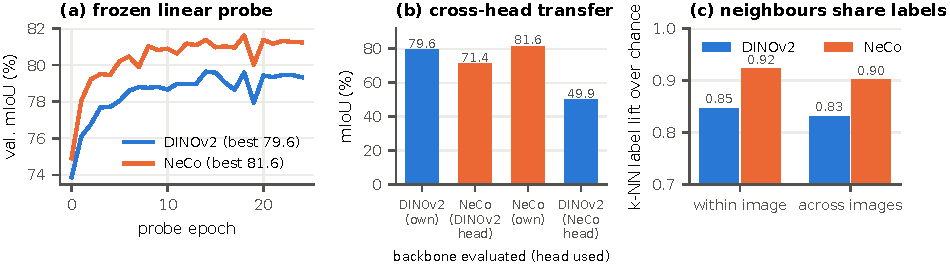
\includegraphics[width=\linewidth]{figs/fig_voc.pdf}
\caption{NeCo vs.\ DINOv2 (ViT-S/14) on PASCAL VOC 2012 under an identical, seed-matched
protocol. \textbf{(a)} Frozen-backbone linear probe: NeCo is ahead from the first epoch
and ends +2.0\,mIoU higher. \textbf{(b)} Neither trained head transfers to the other
backbone, so NeCo changes the representation itself rather than rescaling it. \textbf{(c)}
NeCo's $k$-NN neighbours (k=10) share the query patch's label more often; shown as lift over
the label-prior chance level.}
\label{fig:voc}
\end{figure}

If the NeCo objective were generically too far from downstream tasks, it would also fail
where it was designed to work. We test this with the official code and released weights:
NeCo-post-trained DINOv2 ViT-S/14 against the original DINOv2, evaluated on PASCAL VOC
2012~\cite{everingham2010voc} semantic segmentation with a frozen backbone and a 1$\times$1
linear head. Both runs use the same seed, head initialisation and data order, as in our
P3 comparisons. NeCo reaches 81.6 mIoU against 79.6 (published: 81.4), is ahead from the
first epoch, and has a 5\% (train) and 10\% (val) lower first-epoch loss
(\cref{fig:voc}a). The representation itself changes (\cref{fig:voc}b), and in the
intended direction: NeCo's patch neighbours share the query's ground-truth label more
often, both within images (lift over chance 0.92 vs.\ 0.85) and across images (0.90 vs.\
0.83), and k-means clusters align better with the classes (NMI 0.37 vs.\ 0.33). A gradient-alignment
probe gives a null result in this setting too: the cosine between the NeCo gradient
and the segmentation gradient on the backbone is within noise of zero ($-0.015$ vs.\ a noise
floor of $\pm$0.13). So aligned gradients are not the mechanism anywhere; what matters is
the representation the objective produces once it can actually change the backbone. NeCo's
gradient norm is also only 0.59$\times$ that of the segmentation loss on the same backbone,
a milder version of the ``small encoder signal'' seen in \cref{sec:why-move}.

The contrast pinpoints what is different in TAL. In VOC, NeCo (1) trains a backbone that
\emph{produces} the features, (2) on views that differ at every pixel, (3) for a dense
task where the neighbour structure it optimises is precisely the label structure
being evaluated. In our TAL setting, (1) the features are frozen upstream and only a small
re-mixing encoder is trained, (2) the views are mostly identical, and (3) the task is
sparse, with one verb and two boundaries per segment across 97 classes, so a timestep's
neighbours are not the quantity being evaluated.

\begin{table}[t]
\centering\small
\caption{Summary of the diagnosis. Each candidate explanation for the null result, the
measurement that tests it, and the outcome.}
\label{tab:diagnosis}
\begin{tabular}{>{\raggedright\arraybackslash}p{4.3cm}>{\raggedright\arraybackslash}p{7.5cm}>{\raggedright\arraybackslash}p{3.6cm}}
\toprule
Explanation & Evidence & Verdict \\
\midrule
Head mismatch (P2) & joint fine-tune: gap to control stays $\sim$0.5\pp{} for 6 epochs & ruled out \\
Views carry little signal & 93\% (SF) / 97\% (VM) of level-0 ROI bins see identical input & supported \\
Head absorbs the objective & head moves 12\%, backbone 0.47\%, neck 0.05\% & supported \\
Transferred encoder $\approx$ random init & EMA teacher moves 0.08\%; simulated EMA lag matches measurement & supported (decisive for v1) \\
Init erased by supervised training & CKA to other-seed baseline = seed floor (0.90); no epoch-1 head start & supported \\
Encoder simply under-trained & v2 moves it 20$\times$ more $\Rightarrow$ mAP $-0.95$ & ruled out \\
Objective misaligned with TAL here & post-training and v2 both hurt; VOC control works & supported (setting-specific) \\
NeCo objective weak in general & +2.0 mIoU and label-consistent neighbours on VOC & ruled out \\
\bottomrule
\end{tabular}
\end{table}

%=======================================================================================
\section{Discussion}\label{sec:discussion}
%=======================================================================================

\paragraph{Putting it together.} \Cref{tab:diagnosis} collects the evidence. For the
pre-training protocol as run, the most direct explanation is mechanical. A weak and
partly trivial signal (\cref{sec:why-views}) is absorbed by the head
(\cref{sec:why-move}), the EMA teacher hands on an encoder within $10^{-3}$ of its random
initialisation, and a full supervised schedule moving the encoder by 24\% erases the rest
(\cref{sec:why-erase}). In this regime P3 \emph{cannot} differ from P1 except through
run-to-run noise, and it does not. The more important finding is the second one: when
these obstacles are removed and NeCo does change the encoder, through post-training or
the v2 schedule, the change is harmful. Fixing the EMA schedule would therefore most
likely not turn the null result into a gain. It would turn it into the v2 result.

\paragraph{Lessons for SSL on frozen-feature detectors.} Three lessons generalise beyond
this study. First, \emph{check what is transferred}: with EMA teachers, the momentum
schedule has to be scaled to the number of steps, or the teacher is effectively the
initialisation. Measuring weight movement of the transferred weights is cheap and would
have revealed this immediately. Second, \emph{views must differ where the model looks}.
Crops of a pre-extracted sequence differ only in distant context, so they cannot teach
local invariances. Third, \emph{a single-seed baseline is not a reference}: the 1.4\pp{}
seed range of the SlowFast baseline exceeds every SSL effect we measured, and a
perturbation of $10^{-3}$ in the initialisation is enough to move the final mAP by
0.8\pp.

\paragraph{Limitations.} Seed replicates exist only for SlowFast P1 and P3 ($n{=}3$
each). VideoMAE-L and V-JEPA~2 noise is assumed to match SlowFast's. A
perturbation-matched control, i.e.\ P1 restarted from its initialisation plus random noise of
relative size $8\times10^{-4}$, would quantify the perturbation noise directly. The view-identity
analysis is computed from the architecture rather than measured on activations. The
scene-identity explanation of \cref{sec:why-wrong} is a hypothesis. Only one
dataset and one detector are studied, and we did not try a fully trained encoder
(teacher momentum scaled to the run, no head learning-rate advantage, long schedule).
That configuration is the last untested one, although the v2 trend predicts it would not
help.

\paragraph{What would help instead.} Since information is fixed upstream, the lever is the
features: in this study, switching from SlowFast to EPIC-finetuned VideoMAE-L gained 6.2\pp,
against $<$1\pp{} for any SSL variant. Promising directions are end-to-end or
parameter-efficient backbone adaptation for TAL~\cite{liu2024adatad}, domain-adaptive
self-supervised pre-training of the \emph{backbone} on EPIC video (where pixel-level views
are available and NeCo's assumptions hold), and localization-aware pre-training objectives
such as TSP and BSP~\cite{alwassel2021tsp,xu2021bsp}. If SSL is applied to the TAL encoder
at all, the views should differ in their inputs (e.g.\ feature-space noise, masking or
frame-rate changes), the references should come from within the same video to suppress
scene shortcuts, and the teacher schedule should match the run length.

%=======================================================================================
\section{Conclusion}
%=======================================================================================

NeCo-style self-supervision of ActionFormer's encoder does not improve temporal action
localization on EPIC-KITCHENS-100 verbs. Post-training a converged model hurts
on both feature tracks where it was tested, and the damage persists through joint
fine-tuning. Pre-training is indistinguishable from the baseline on all three tracks
once seed noise is taken into account. The reasons are, in order: views of a
pre-extracted sequence are mostly identical inputs; the projection head absorbs the
objective; the EMA teacher that is transferred has barely left its random
initialisation; supervised training erases what remains; and when the encoder is forced
to change, it changes in a direction that hurts localization. In NeCo's own dense-image
setting the objective works as published, so the negative result is a statement about
self-supervising a re-mixing encoder over frozen, already-supervised features for a
sparse temporal task, not about neighbour-consistency learning in general.

\small
\bibliographystyle{unsrtnat}
\bibliography{refs}

\end{document}
